\documentclass[alternative-exam.tex]{subfiles}
\begin{document}

\chapter{Tussentijdse Toets}

\section{Vraag}
Professor Veys geeft een tussentijdse toets voor Lineaire Algebra in week 9 van het eerste semester.
Hij wil rekening houden met de voorkeuren van alle richtingen die deze toets krijgen. De jaarverantwoordlijken van wiskunde, fysica en informatica geven hun voorkeuren door. De voorkeuren zien er als volgt uit.\\\\
De wiskundigen gaan graag naar de winabar en willen daarom de toets liefst niet op donderdag. De fysici hebben op dinsdag een andere tussentijdse toets en zouden het liefst minstens één dag na die toets geen toets hebben, zodat ze tijd hebben om te studeren. De informatici willen de toets liefst niet op maandag, omdat er dan een deelexamen van SOCS plaatsvindt. Geen enkele richting wil de toets op vrijdag, omdat ze op donderdag willen uitgaan.\\\\
Professor Veys zet het liefst de toets voor de informatici als eerst, omdat die verbetering het langst duurt. Bovendien wil hij niet dat de drie toetsen op dezelfde dag vallen maar hij wil ook niet er dagen tussen de toetsen zijn. Hij wil dus de drie toetsen op drie opeenvolgende dagen zetten.\\\\
Hoe plant Professor Veys best de tussentijdse toets voor de drie richtingen?

\section{Modeloplossing}
We lossen dit probleem om met constraint processing technieken. We zullen de beperkingen formeel defini\"eren, en er een constraint processing oplossingsmethode op uitvoeren.
\subsection{Formele formulering}
\begin{figure}[H]
\centering
\caption{Waarden voor dagen}
\label{waarde_dagen}
\begin{tabular}{| c | c | }
\hline
dag & waarde\\
\hline
maandag & 1\\
dinsdag & 2\\
woensdag & 3\\
donderdag & 4\\
vrijdag & 5\\
\hline
\end{tabular}
\end{figure}
We kiezen drie variabelen. Noem $z_f$, $z_w$, $z_i$ respectievelijk de dag waarop fysica, wiskunde en informatica de toets krijgt. Om de beperkingen makkelijk op te schrijven wijzen we aan elke dag van maandag tot vrijdag in week 9 (de dagen dat er een toets gegeven kan worden) een getal toe zoals beschreven in figuur \ref{waarde_dagen}.
Nu kunnen we de constraints formuleren volgens deze waarden.

\subsubsection{Unaire beperkingen}
Geen enkele richting wil hun toets op vrijdag. Dit kunnen we formuleren als volgt.
\[z_f \neq 5,\ z_w \neq 5,\ z_i \neq 5\]
De Wiskundigen willen hun toets niet op donderdag.
\[
z_w \neq 4
\]
De fysici willen hun toets ten vroegste twee dagen na dinsdag.
\[
z_f > 3
\]
Tenslotte willen de informatici de toets niet op maandag.
\[
z_i \neq 1
\]
We kunnen nu de unaire beperkingen als volgt samenvatten.
\[
\left\lbrace
\begin{array}{c c c}
c(z_w) & \leftrightarrow & z_w \neq 5 \wedge z_w \neq 4\\
c(z_f) & \leftrightarrow & z_f \neq 5 \wedge z_f > 3\\
c(z_i) & \leftrightarrow & z_i \neq 5 \wedge z_i \neq 1\\
\end{array}
\right.
\]
\subsubsection{Binaire beperkingen}
Professor Veys zorgt voor de binaire constraints. Hij wil de toets als eerst aan de informatici geven.
\[
z_i < z_w,\ z_i < z_f
\]
Tenslotte wil hij dat elke toets op een andere dag valt en dat er geen dagen tussen twee toetsen zitten.
\[
z_i \neq z_w,\ z_i \neq z_f,\ z_w \neq z_f
\]
\[
|z_i - z_w| \le 2,\ |z_w - z_f| \le 2,\ |z_i - z_f| \le 2
\]
De binaire beperkingen vatten we nu als volgt samen
\[
\left\lbrace
\begin{array}{c l l c c c c}
c(z_w, z_f) & \leftrightarrow && & z_w \neq z_f &\wedge& |z_w - z_f| \le 2\\
c(z_f, z_i) & \leftrightarrow & z_i < z_f &\wedge& z_i \neq z_f &\wedge& |z_i - z_f| \le 2\\
c(z_i, z_w) & \leftrightarrow & z_i < z_w &\wedge& z_i \neq z_w &\wedge& |z_i - z_w| \le 2\\
\end{array}
\right.
\]

\subsection{Domein}
Het domein van de variabelen bespreek ik als laatst omdat dit nog verkleind kan worden als we rekening houden met node consistentie.
Aanvankelijk hebben alle variabelen het domein $d_\bullet = \{1,2,3,4,5\}$. Door rekening te houden met de unaire beperkingen van variabelen kunnen we hun domein kleiner maken.
\[
\left\lbrace
\begin{array}{r l}
d_{z_w}' &= \{1,2,3,5\}\\
d_{z_f}' &= \{4,5\}\\
d_{z_i}' &= \{2,3,4,5\}\\
\end{array}
\right.
\]

\subsection{Constrant network}
\begin{figure}[H]
\caption{Constraint Network}
\label{fig:fourTeachersConstraintNetwork}
\centering
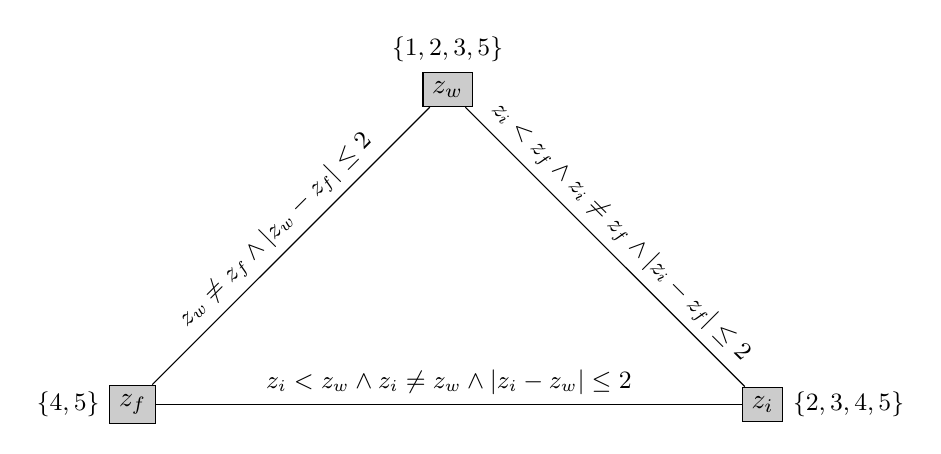
\begin{tikzpicture}[vari/.style={fill=black!20,rectangle,draw=black}]
\def\dx{4};
\def\dy{4};
\def\r{0.125};
\node[vari] (A) at (0,\dy) {$z_w$};
\node[vari] (B) at (-\dx,0) {$z_f$};
\node[vari] (C) at (\dx,0) {$z_i$};

\node[anchor=south] (DA) at (A.north) {\small{$\left\{1,2,3,5\right\}$}};
\node[anchor=east] (DB) at (B.west) {\small{$\left\{4,5\right\}$}};
\node[anchor=west] (DC) at (C.east) {\small{$\left\{2,3,4,5\right\}$}};

\draw (A) to node[midway,sloped,above]{\small{$z_w \neq z_f \wedge |z_w - z_f| \le 2$}} (B);
\draw (A) to node[midway,sloped,above]{\small{$z_i < z_f \wedge z_i \neq z_f \wedge |z_i - z_f| \le 2$}} (C);
\draw (B) to node[midway,sloped,above]{\small{$z_i < z_w \wedge z_i \neq z_w \wedge |z_i - z_w| \le 2$}} (C);
\end{tikzpicture}
\end{figure}
Als samenvatting van heel het probleem kunnen we het zogenaamde constraint network opstellen. Zie figuur \ref{fig:fourTeachersConstraintNetwork}.

\subsection{Uitwerking van de oplossingsmethode}
We zullen nu de methode 'forward checking' toepassen op dit probleem. Omwille van effici\"entie zullen we een zogenaamde dynamic search rearrangement techniek toepassen. We zullen op elk niveau de waarde kiezen met het kleinste overgebleven domein kiezen om een waarde aan toe te kennen.



\end{document}